\section{A supervised model of dyadic sentiment}

\label{section:foreign_relations_supervised_model}

In the last chapter we described a model for identifying influential
documents.  An important feature of that model was that it was
unsupervised; only after it was fit did we compare the inferred
influence of an article with the number of citations it had recieved.
In this section we will take a more direct approach, fitting a
model with labels \emph{defined} to represent sentiment.

Here will make further assumptions about the object of discussion in
the text. We will assume in particular that each country can be
described by a vector in some latent space.  The relationship between
two countries is then determined (up to stochasticity) by the
relationship between these countries' positions in this latent space
(models that make this assumption are sometimes referred to as latent
space models or spatial models).  A spatial a model provides two
benefits for us. First, it provides interpretability: nations with similar
positions in this latent space tend to interact more positively, while
nations further apart tend to have more tension in their relationship.
A spatial model also allows us to draw on existing work from
multidimensional scaling, which has been used successfully in both
political science \cite{martin:2002,jackman:2001} and social network
modeling \cite{hoff:2002,chang:2009}.

\subsection{Inferring sentiment from text.}
\label{section:text_regression}
When a news source discusses the relationship between these nations,
the author's choice of words $\bm w_d$ reflects the relationship
between the countries.  We model this sentiment with the text of the
article $d$.  Using text regression \cite{kogan:2009}, we model
sentiment using the wordcounts $\bm w_d$ of the article:
\begin{align}
  s_d | \bm w_d, \beta \sim \mathcal{N}( \bm w_d^T \beta, \sigma_W^2 ).
  \label{eq:sentiment_text}
\end{align}
For the purposes of countries' positions in the latent-space model, we
will assume that $\beta$ is observed (we describe how to fit $\beta$
with \myeq{sentiment_text} and human labels in
Section~\ref{section:mturk}).  In fitting $\beta$, we interpret the
distribution of $s_d$ as a Gaussian with a mean which depends on the
text.

\subsection{A temporal model of interaction.}
We formalize the latent space assumption by letting each country $c$
take a position $\bm x_c \in \mathbb{R}^p$ in a space of latent
political sentiment. The relationship between two countries $c_1, c_2$
will be described by a scalar $s_{c_1,c_2} \in \mathbb{R}$.  This
sentiment is determined by the interaction of their positions:
$s_{c_1, c_2} = \mathcal{F}(\bm x_{c_1}, \bm x_{c_2})$, for some
suitable function $\mathcal{F}$.

\begin{figure}
  \center
  \vspace{-55pt}
  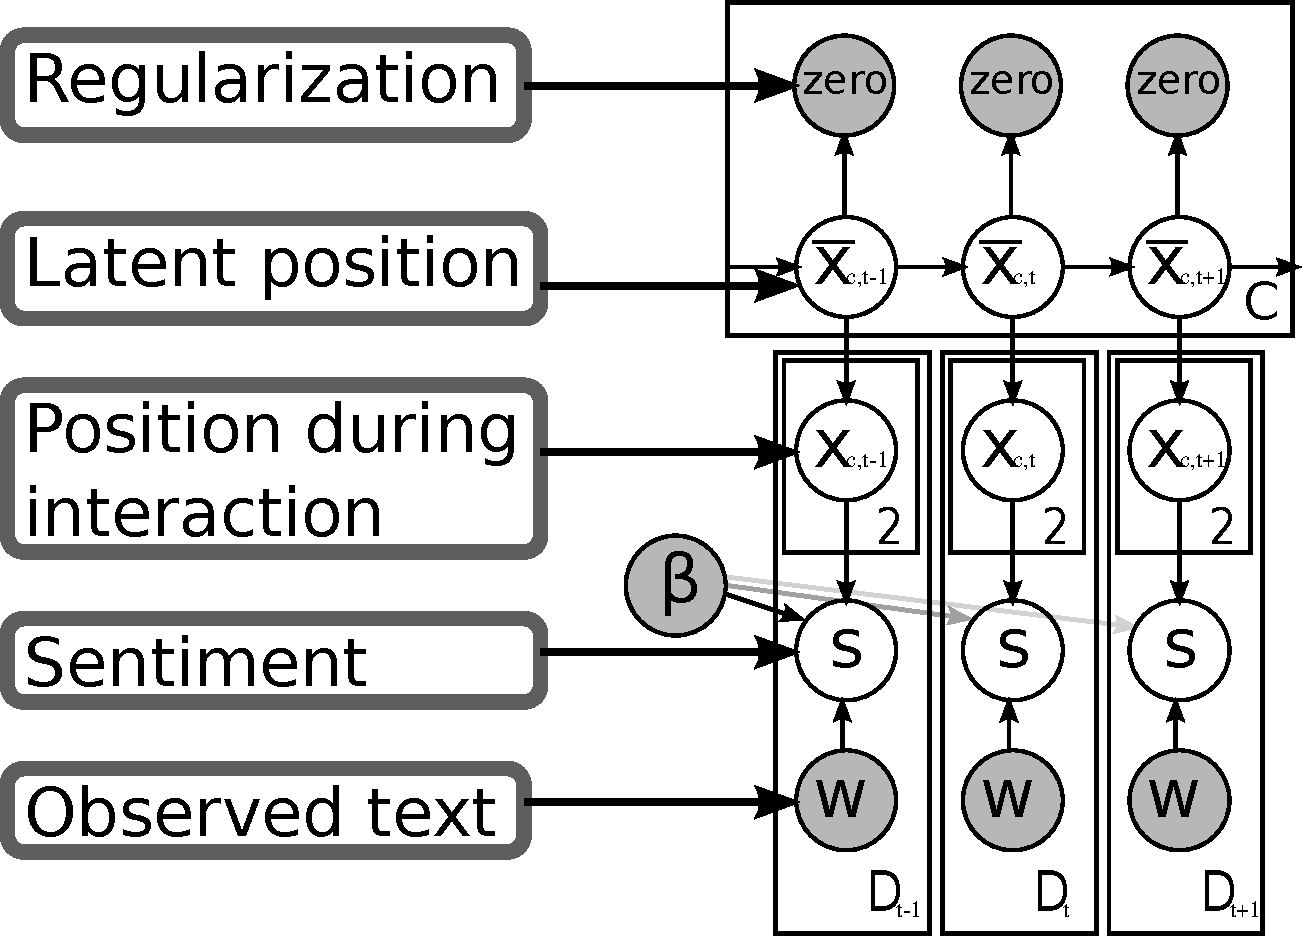
\includegraphics[width=0.5\textwidth]{chapter_foreign_relations/figures/countries_gm.pdf}
  \caption{A time-series model of countries' interactions.
    Pseudo-observations of ``zero'' are added for regularization.
    Amazon Mechanical Turk labels are used to fit $\beta$, which is
    used to infer unobserved sentiments.}
  \label{figure:gm}
\end{figure}


Foreign relations are not static; nations' alliances and preferences
change over time with the evolution of economies, technology, and
culture.  Therefore we make this a fully temporal model by
allowing each country's mean position $\bar x_{c,t}$ to drift over
time with the Markov transition
\begin{align}
  \bar x_{c,t} | \bar x_{c,t-1} \sim \mathcal{N}(\bar x_{c,t-1}, \sigma_{\mbox{\tiny chain}}^2),
\end{align}
as shown in Figure~\ref{figure:gm}. At any time $t$, state $c_1$ may interact with state $c_2$ in the following way:
\begin{align}
  x_{c_1,d} \sim \mathcal{N}(\bar x_{c_1, t}, \sigma_D^2) \nonumber \\
  x_{c_2,d} \sim \mathcal{N}(\bar x_{c_2, t}, \sigma_D^2) \nonumber \\
  s_d := x_{c_1,d}^T x_{c_2,d}, \label{eq:sentiment_space}
\end{align}
where we interpret $s_d$ as the sentiment between $c_1$ and $c_2$ as
reflected by article $d$.  When $c_1$ and $c_2$ are similar (as
measured by their inner product), their sentiment $s_d$ will be
positive; if they are dissimilar, their sentiment will be negative.
More extreme values indicate stronger sentiment.

For the purposes of countries' positions in the latent-space model,
however, we will use the symmetry of the Gaussian to model text as if
it were conditioned on sentiment: $\mathcal{N}(s_d | \bm w_d^T \beta,
\sigma_w^2) = \mathcal{N}( \bm w_d^T \beta | s_d, \sigma_W^2 )$.  This
allows us to reconcile \myeq{sentiment_text} and
\myeq{sentiment_space}, so that the distribution of sentiment
conditioned on text and countries' positions is:
\begin{align}
  p(s_d | \bm w_d, \beta, x_{c_1,d}, x_{c_2,d}) & \propto
  \mathcal{N}(\bm w_d^T \beta | s_d, \sigma_W^2 )
  \mathcal{N}(x_{c_1,d} | \bar x_{c_1, t}, \sigma_D^2)
  \mathcal{N}(x_{c_2,d} | \bar x_{c_2, t}, \sigma_D^2) \nonumber \\
  & \hspace{20pt} \mbox{ such that } s_d = \mathcal{F}(x_{c_1,t},
  x_{c_2,t}) \nonumber \\
  & = 
  \mathcal{N}(\bm w_d^T \beta |
    \mathcal{F}(x_{c_1,t}, x_{c_2,t}), \sigma_W^2 )
  \mathcal{N}(x_{c_1,d} | \bar x_{c_1, t}, \sigma_D^2)
  \mathcal{N}(x_{c_2,d} | \bar x_{c_2, t}, \sigma_D^2).
\end{align}

% In addition, a UN resolution may come up for vote at any time.  States
% cast a vote based on their current positions:
% \begin{align}
% x_{c_1,d} \sim N(\bar x_{c_1, t}, \sigma_D^2) \nonumber \\
% p(v_{cr}) = \sigma(x_{c_2, t} b_r + a_r) \nonumber \\
% \end{align}

% \begin{wrapfigure}{r}{0.4\textwidth}
%   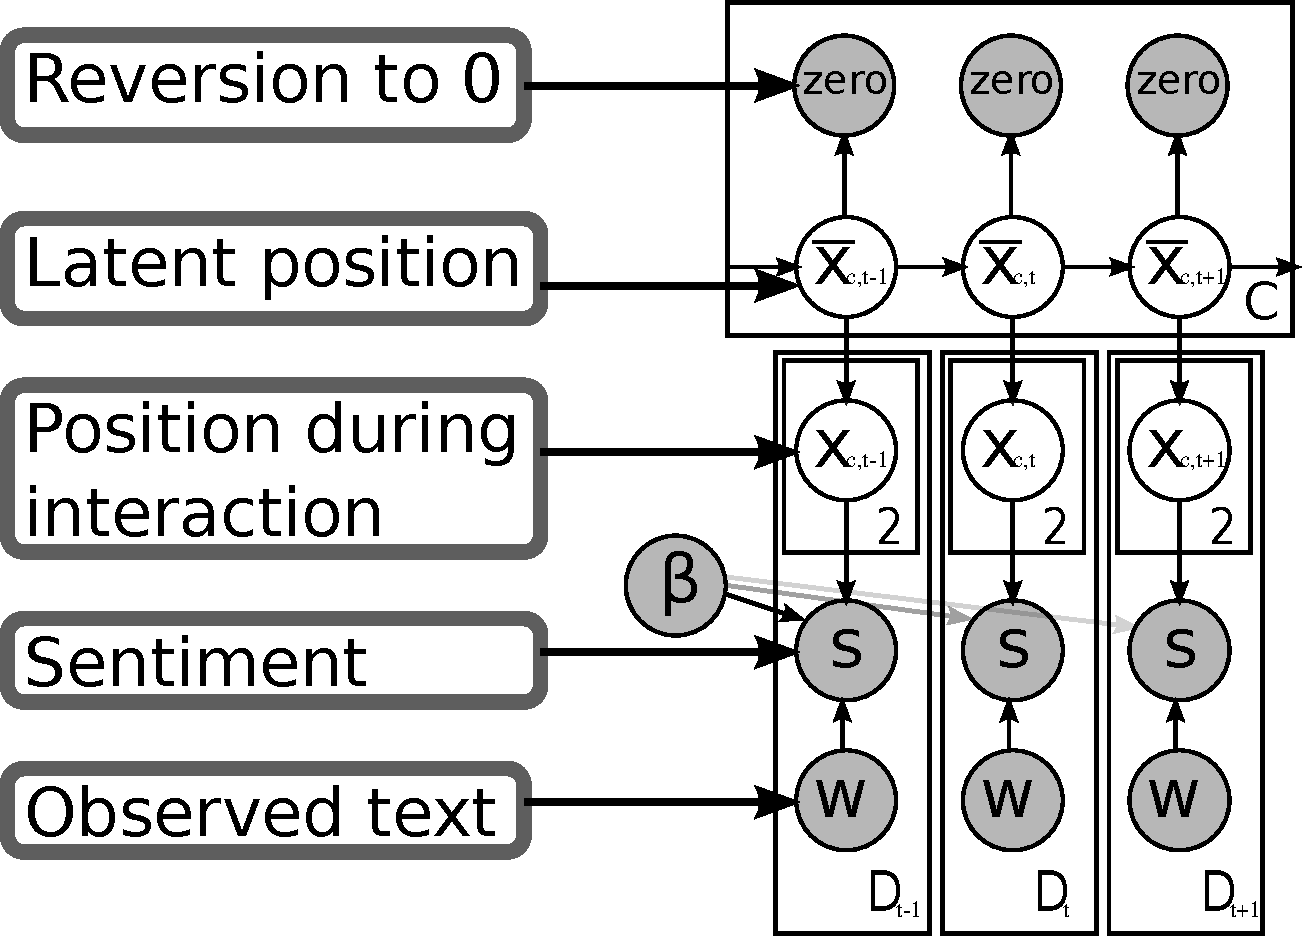
\includegraphics[width=0.4\textwidth]{figs/countries_gm.pdf}
%   \caption{The full time-series model of interaction by countries.
%     The large plate shows replication of a Markov chain for each
%     country.  Certain countries interact at each epoch -- possibly
%     multiple times -- with sentiment $s$.}
%   \label{fig:countries_by_ip}
% \end{wrapfigure}

\paragraph{A brief comment on notation.} Before proceeding to
inference and the experimental validation of this model, we pause to
summarize our use of notation.  In this chapter, we will use notation
flexibly when it is convenient.  The typical unit of discussion will
be the $d$th document occurring at time $t$.  The $d$th document
discusses two countries, $c_1$ and $c_2$; these define a tuple $(\{
c_1, c_2 \}, d, t)$ (where the set $\{ c_1, c_2 \} = \{ c_2, c_1 \}$).
We will generally use $d$ to index documents, $t$ or $s$ to index
time, and $c$ to index a country.  When document $d$ is given, we may
refer to its time $t_d$ (which is unique) or to the two interacting
countries as $c_{d,1},c_{d,2}$ or $c_1,c_2$.  Alternatively, we may
refer to the documents in which a country $c$ appears as $d_{c,1},
\ldots, d_{c,1}$.  For example, we may index the variable
$x_{(c_1,d,t)}$ variously as $x_{c_{d,1}}$ or $x_{d,1}$, or even $x_c$
if the context is clear. The sentiment between two countries might be
described as $s_d$, $s_{c_1,c_2}$, $s_{d,t}$, or $s_{c_1,c_2,d,t}$.

\subsection{Related work}

% Democracy, Political Similarity, and International Alliances, 1816-1992
% Brian Lai
% Dan Reiterb
% Department of Political Science, Emory University
Spatial models such as Item Response Theory (IRT) have been developed
over the past century by quantitative social scientists for analyzing
behavior.  While much of this work has been used to model
parliamentary voting behavior, these techniques have also been used to
model voting in the UN General Assembly. Gartzke et al., for example,
use these votes and alliance models to study the nations' affinities
\cite{gartzke:1998}.

These models have been developed for dyadic data more fully in network
models such as the latent space model \cite{hoff:2002,sarkar:2005}, in
which the probability of a link between two nodes is a function of
their latent-space distance.  The qualitative relationship of
entities' dyadic relationships has been more fully developed with text
by the relational topic model, which uses free text to model the
relationship between actors in an unsupervised setting
\cite{chang:2009}.
% Supervised topic models


% Affinity of states dataset: 
% Fading Friendships (working paper)
% Alliances, Affinities and the Activation of International Identities∗
% Erik Gartzke†
% Alex Weisiger‡
% 7 March 2011

\subsection{Inference}
We fit the \emph{MAP} objective of this probabilistic model.  This has
the benefit of both clean exposition and simple implementation, and it
can be interpreted as a form of unregularized variational inference.
We optimize the \emph{MAP} objective in this model using an
expectation maximization (EM) algorithm.

We designed the probabilistic objective to make inference tractable.
For example, the Gaussian distribution of per-document sentiment
variables $x_{c, t} | \bar x_{c,t}$ makes inference for $\bar x_{c,t}$
closed-form.  Countries' per-interaction positions $x_{c_{d,1}, t},
x_{c_{d,2},t} | \bar x_{c_{d,1},t}, \bar x_{c_{d,2}, t}, s_{c_{d1},
  c_{d2}}$ are then fit using gradient ascent.

Our goal in performing EM is to estimate parameters for the model.  Expectation allows us to find a \emph{MaP} estimate by optimizing the lower bound on the data likelihood:
\begin{align}
  \mathcal{L_{x}} \log p(s_d, \bm w, \beta, x)
  % & \propto p(s_d | \bm w, \beta, x, \beta) \\
  & \ge \log \expectq{ \frac{q(\bar x)}{q(\bar x)}
    p(s_d | \bm w, \beta, x, \beta) } \nonumber \\
  & \ge \expectq{ q(\bar x)
    \log \frac{ p(s_d | \bm w, \beta, x, \beta) }{
      q(\bar x)} }
\end{align}

\subsubsection{M Step.} In the M step, we estimate the mean $\bar
x_{c,t} | x_{c_1,1}, \ldots, x_{c_N,T}$ of each country's position
using a modified Kalman filter (modified because it must take into
account all interactions in a given year).  This step differs from a
standard Kalman filter in that we may have no or multiple observations
on any given date.\footnote{We also experimented with
  \emph{pseudo-observations} for each country at each day $t$ with
  mean 0 and variance $\sigma_p^2$.  These observations are a form of
  ``time-series regularization'' and reflect the sense that a lack of
  news is effectively neutral news.  Low values of $\sigma_p^2$ harmed
  performance, and it was best set around $10^6$.}  The prior over the
ends of the chain are standard normal.

\paragraph{Kalman updates.}
The M step seeks the expected value of the mean position $\bar x_c$
for each country $c$ given our estimate of the $D_{c,s}$ interactions
at each time $s=1, \ldots, T$:
\begin{align}
  \arg \max \bar x_{c,t} | x_{c,1,1}, \ldots, x_{c,D_{c,1},1}, x_{c,D_{c,2},2},
  \ldots, x_{c,D_{c,t},T},
\end{align}
for $t=1, \ldots, T$. The optimal value for $\bar x$ can be found with
a modified Kalman smoother \cite{kalman:1960}.  This modified Kalman
smoother requires a forward filter step and a backward filter step.
The forward filter estimates the mean position given all previous
observations (note that we use $x_{c,d,t}$ to describe the position of
country $c$ at time $t$ for interaction $d$:
\begin{align}
  \bar x_{\mbox{\tiny forth},c,t} | \bar x_{\mbox{\tiny forth},c,t-1}, \{ x_{c,d,t-1} \}_{d}
  & \gets \frac{\bar x_{\mbox{\tiny forth},c,t-1} / \sigma_{\mbox{\tiny forth},t-1}^2
    + \sum_{d=1}^{D_{c,t-1}} x_{c,d,t-1} / \sigma_{\mbox{\tiny obs}}^2}
  {1 / \sigma_{\mbox{\tiny forth},t-1}^2 + 1 / \sigma_{\mbox{\tiny obs}}^2} \\
  \sigma_{\mbox{\tiny forth},t}^2
  & \gets \frac{1}{1 / \sigma_{\mbox{\tiny forth},t - 1}^2
    + D_{c,t-1} / \sigma_{\mbox{\tiny obs}}^2} + \sigma_{\mbox{\tiny chain}}^2,
\end{align}
with initial condition $\bar x_{c,0} = 0,
\sigma_{\mbox{\tiny forth},0}^2=10$.  The backward step estimates
the chain's mean given all current and future observations:
\begin{align}
  \bar x_{\mbox{\tiny back},c,t} | \bar x_{\mbox{\tiny back,c,t+1}}, \{ x_{c,d,t} \}_d
  & \gets \frac{\bar x_{\mbox{\tiny back},c,t+1} / \sigma_{t+1}^2
    + \sum_{d=1}^{D_{c,t}} x_{c,d,t} / \sigma_{\mbox{\tiny obs}}^2}
  {1 / \sigma_{\mbox{\tiny back},t-1}^2 + 1 / \sigma_{\mbox{\tiny obs}}^2} \nonumber \\
  \sigma_{\mbox{\tiny back},t}^2
  & \gets \frac{1}{1 / (\sigma_{\mbox{\tiny back},t + 1}^2 + \sigma_{\mbox{\tiny chain}}^2)
    + D_{c,t} / \sigma_{\tiny obs}^2},
\end{align}
with initial conditions $\bar x_{\mbox{\tiny back},c,T} = 0, \sigma_{\mbox{\tiny
    backward},T}^2=10$. The smoothed means---that is, the mean of countries' positions at time $t$ given all observations for all time---are
\begin{align}
  \expectq{\bar x_{c,t}} & = \bar x_{c,t} | x \nonumber \\
  & = \bar x_{c,t} | \bar x_{\mbox{\tiny forth,c,t}}, \bar x_{\mbox{\tiny back,c,t}}, \sigma_{\mbox{\tiny back}}^2, \sigma_{\mbox{\tiny forth}}^2 \nonumber \\
  & = \frac{\bar x_{\mbox{\tiny forth},c,t} / \sigma_{\mbox{\tiny forth},t}^2
    + \bar x_{\mbox{\tiny back},c,t} / \sigma_{\mbox{\tiny back},t}^2}
  {1 / \sigma_{\mbox{\tiny forth},t}^2
    + 1 / \sigma_{\mbox{\tiny back},t}^2}
\end{align}

% x_{c,d,t}
\subsubsection{E Step.} In the E-step, our goal is to infer each
nation's position $x_{c_{d,1}} | \expectq{ \bar{x}_{c,d,t} },
x_{c_{d,2}}, s_d$ during interaction $d$ given its expected mean $\expectq{ \bar
x_{c_{d,1},t_d} }$ and the text $\bm w_d$ describing this interaction,
\emph{and} given the other country's position for this interaction.
We find these positions by gradient ascent on each interaction:
\begin{align}
  & {\arg \max}_{x_{c_{d,1},t}, x_{c_{d,2},t}}
  p(\bm w_d^T \beta | \mathcal{F}(x_{c_{d,1},t}, x_{c_{d,2},t}),
  \expectq{ \bar x_{c_{d,1},t} }, \expectq{ \bar x_{c_{d,2},t} }) \nonumber \\
  & = 
  {\arg \max}_{x_{c_{d,1},t}, x_{c_{d,2},t}}
  p(\bm w_d^T \beta | \mathcal{F}(x_{c_{d,1},t}, x_{c_{d,2},t}), \beta)
  p(x_{c_{d,1},t} | \expectq{ \bar x_{c_{d,1},t} } )
  p(x_{c_{d,2},t} | \expectq{ \bar x_{c_{d,2},t} } ).
\end{align}

\subsection{Empirical studies: comparisons with ground truth}
We now turn to an experimental analysis of this model.  We first
describe the human labels we have used to define sentiment $s_d$
within this model.  We then describe two news archives from which we
have inferred countries' sentiment over time. text in which the
relationships of countries are deto which we applied this model and .
We then turn

\subsection{Sentiment labels $s$}
\label{section:sentiment_models}

To infer the sentiment $s_d$ between two countries, we treat the
corresponding news article as a bag of words and fit text regression
\cite{kogan:2009} to predict the sentiment from the text.  We used two
sources for sentiment labels: Amazon Mechanical Turk and Covariates of
War.  In each case, we fit a text regression which predicted the
sentiment $s_d$ from a training set of text snippets.

\subsection{Datasets and tokenization}

\paragraph{New York Times.}
We fit and evaluate this model over news articles discussing 245
nations and territories from twenty years of the \emph{New York Times}
(NYT).  This collection spanned the years 1987 to 2007, a period which
included both Gulf wars; the collapse of the Soviet Union; the
reunification of Germany; September 11th, 2001; and countless other
world events.

\paragraph{Data preparation.}
We used articles from the Foreign, Business, Financial, and Magazine
desks of the newspaper during this period. We made an important
assumption that the scope of foreign sentiment discussion is at the
level of a paragraph.  We therefore used the subset of paragraphs
which discuss exactly two nations as ``documents'' $d$, a collection
of 257,472 paragraphs from 1987 to 2007.  We then defined a vocabulary
to be those words which appeared at least twenty times in the
collection, in no more than 40\% of documents, and in at least 0.1\%
of documents.

This resulted in a vocabulary of 5958 words, mentioned by 40,356
paragraphs. We randomly selected 80\% (32,249) distict paragraphs from
this set as training examples and used the remaining examples to
evaluate our model.

We next labeled our training examples with both human reviewers and
expert labels, representing opposite ends of the extreme.

\subsubsection{Amazon Mechanical Turk labels}
\label{section:mturk}

\emph{Amazon Mechanical Turk} (AMT) is a crowdsourcing platform which
provides a \emph{requestor} (the author of this thesis) with access to
thousands of \emph{workers} who perform simple tasks over the
Internet.  Although the requestor can use tests to ensure that workers
are high-quality, these workers are typically not experts.

\begin{figure*}
  \setlength\fboxsep{0pt}
  \setlength\fboxrule{0.5pt}
  \center \fbox{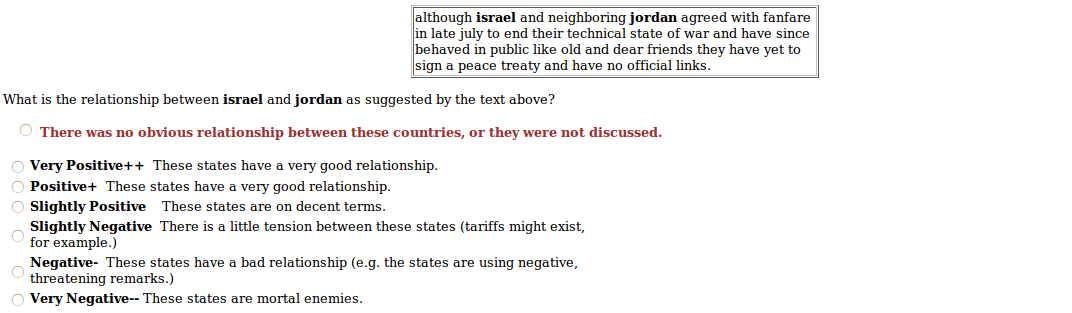
\includegraphics[width=1.0\textwidth]{chapter_foreign_relations/figures/mturk_screenshot.png}}
  \label{figure:mechanical_turk_sample}
  \small\caption{A screenshot of a Mechanical Turk labeling task.
    Sometimes relationships may be complicated; both raters gave this
    example a score of ``slightly positive''.}
  \normalsize
\end{figure*}

To fit the model, we asked \emph{Amazon Mechanical Turk} raters to
rate the sentiment between two nations mentioned in the text of a
paragraph on the scale -5 (mortal enemies), $\ldots$, 5 (very good
relationship). We illustrate a rating task (as seen by a Mechanical
Turk worker) in \myfig{mechanical_turk_sample}.

Raters were asked to review a random subset of 3607 paragraphs from
the original collection.  Before fitting the model, we manually
disqualified eight raters (out of 85) who consistently performed
poor ratings.

With all rated paragraphs which were not in the test set, we fit the
coefficients $\bm \beta$ of the text regression discussed in
Section~\ref{section:model}.  This coefficient was then treated as
constant in the joint model in Figure~\ref{figure:gm} to allow us to
infer sentiment from the words of all 32,249 training paragraphs.  We
illustrate the $\bm \beta$ inferred from Mechanical Turk-labeled
paragraphs in \myfig{fr_example_betas} (left).

\subsubsection{Expert labels: Correlates of War}
\label{section:correlates_of_war}

We also used a combined set of expert labels based on the Correlates of War \cite{sarkees:2010} and Issue Correlates of War \cite{hensel:2001}.
\begin{itemize}
  \item The \emph{Correlates of War} project ``seeks to facilitate the
    collection, dissemination, and use of accurate and reliable
    quantitative data in international relations''
    \cite{cow_webpage:2012}, and it provides labels describing the
    relationships between pairs of countries from 1823 to 2003.
    At-war is a binary relationship (either countries are at war, or
    they are at peace). We used a list of CoW inter-state wars
    (version 4.0) from 1823 to 2003 of inter-state wars
    \cite{sarkees:2010}.
  \item The \emph{Issue Correlates of War} project ``is a research
    project that is collecting systematic data on contentious issues
    in world politics'' \cite{icow_webpage:2012}, and they provide
    expert labels on a variety of inter-state conflicts that \emph{do
      not require militarized conflict}.  However, these issue label
    do require documented evidence of contention between states; such
    issues include maritime and territorial disputes.
    \cite{icow_webpage:2012,hensel:2001}.
\end{itemize}

We combined these datasets by treating two countries as having a
rating of -5 if they are at war from the Correlates of War codes and
-1 if there is any contentious issue between the countries in the
Issue Correlates of War.\footnote{These values were selected to
  correspond roughly to the Mechanical Turk labels.}.  All other pairs
of countries were treated as having a rating of 0.1.  As before, we
fit the text regression parameters $\beta$ using these labels on the
training set and evaluated countries' ratings on the test dataset. We
illustrate $\bm \beta$ fit to CoW-labeled paragraphs in
\myfig{fr_example_betas} (left).

\begin{figure}
  \begin{tabular}{cc}
    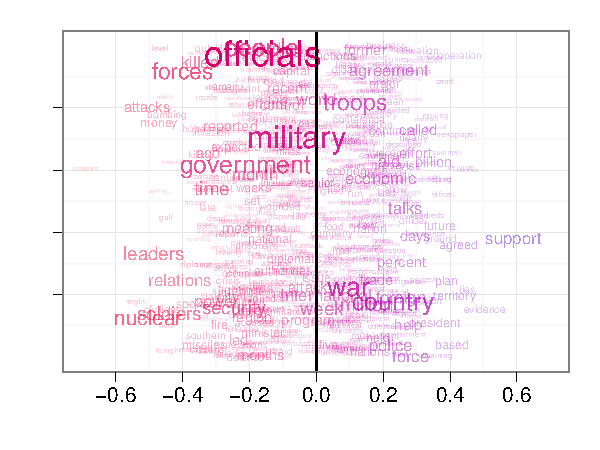
\includegraphics[width=0.4\textwidth]{chapter_foreign_relations/figures/mturk_sample_words.pdf} &
    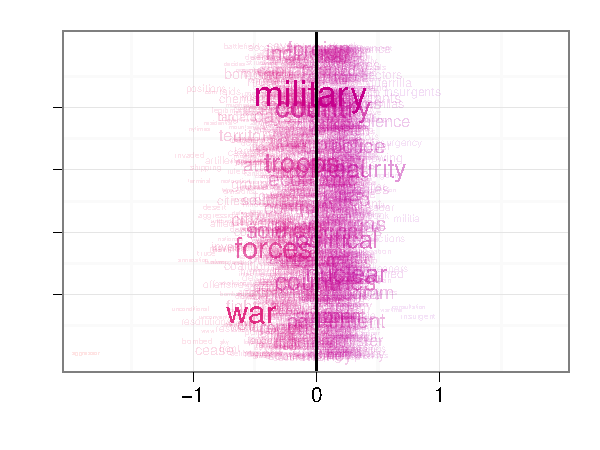
\includegraphics[width=0.4\textwidth]{chapter_foreign_relations/figures/cow_sample_words.pdf} \\
    \end{tabular}
  \caption{Coefficients $\beta_w$ for selected words $w$ fit on text
    labeled by Amazon Mechanical Turk workers (left) and Correlates of
    War data (right). Coefficients fit from Mechanical Turk labels are
    more clearly separated than those fit to Correlates of War labels;
    this is likely due to explicit positive sentiment in that dataset.
    The $x$-axis is $\beta$, and the $y$-axis is used for display (it
    corresponds to no variable).  Size of each word is proportional to
    $\sqrt{\mbox{frequency}}$, and color corresponds to $\beta$.}
  \label{figure:fr_example_betas}
\end{figure}

\subsubsection{Casual vs. expert labels}
The CoW represent a data source which is fairly different from
Mechanical Turk ratings. In the NYT dataset, CoW ratings and
Mechanical Turk ratings were correlated at $\sigma=0.196$.  To
see why this was the case, we give several examples:
\begin{itemize}
  \item $s_{d,\mbox{AMT}} = 1, s_{d,\mbox{CoW}}=-5$. \emph{as an
    indication of the dangers the damage occurred in waters where
    military spokesmen said no mines had been suspected before but
    where a \textbf{saudi} officer said today that some 22 were later
    found. \textbf{iraq}i mines widely deployed} \cite{cushman:1991}
  \item $s_{d,\mbox{AMT}} = -5, s_{d,\mbox{CoW}}=0.1$ \emph{not since
    the grim old days of the cold war have relations between the
    \textbf{united states} and russia been quite as problematic as they
    are this weekend on the eve of president clinton's visit for
    celebrations marking the 50th anniversary of the allied victory in
    europe in world war ii.} \cite{apple:1995}
\end{itemize}

The first of these examples outlines a limitation in the ratings we
obtained: a single paragraph is sometimes too small a unit of
discussion.  This meant Mechanical Turk workers likely missed the
larger context of the article about the Gulf war (including the title,
\emph{War in the Gulf: Sea Mines; Allied Ships Hunt Gulf for Iraqi
  Mines}).

The second example represents a limitation of both data sources.  The
two Mechanical Turk ratings of -5 were clearly too strong, as the
countries are not at war; but AMT workers likely based their rating in
part on the reference to World War II (worker instructions deserve a
rating of -3 or, possibly -1).  In addition, however, the United
States and Russia were not at War and had no official, documented
conflicts at this time.  This means that this sentiment was not
reflected in the CoW labels -- which defaulted to 0.1.

\label{section:experiments}

\subsubsection{Results}
 \begin{figure}
  \begin{tabular}{ccc}
    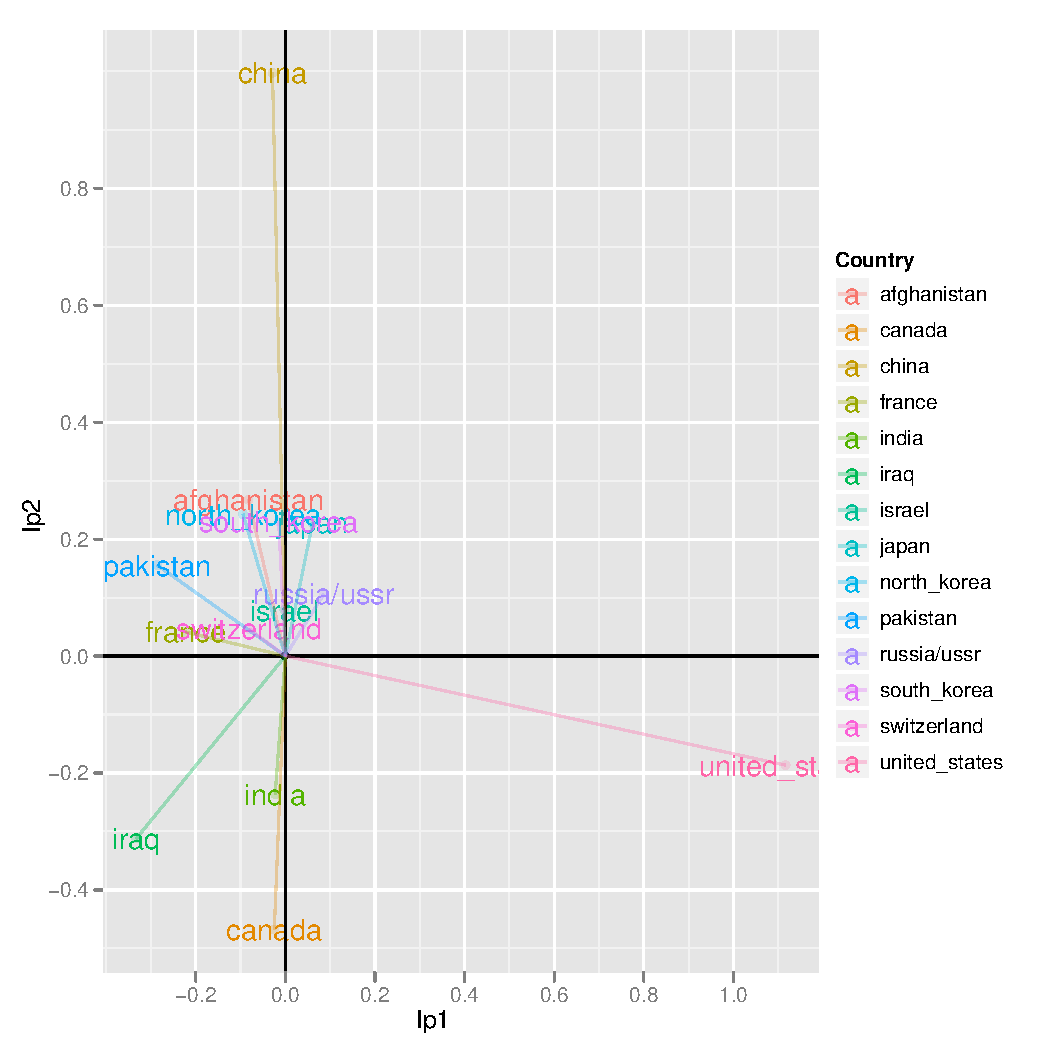
\includegraphics[width=0.33\textwidth]{chapter_foreign_relations/figures/002_countries_by_ip_1987.pdf} &
    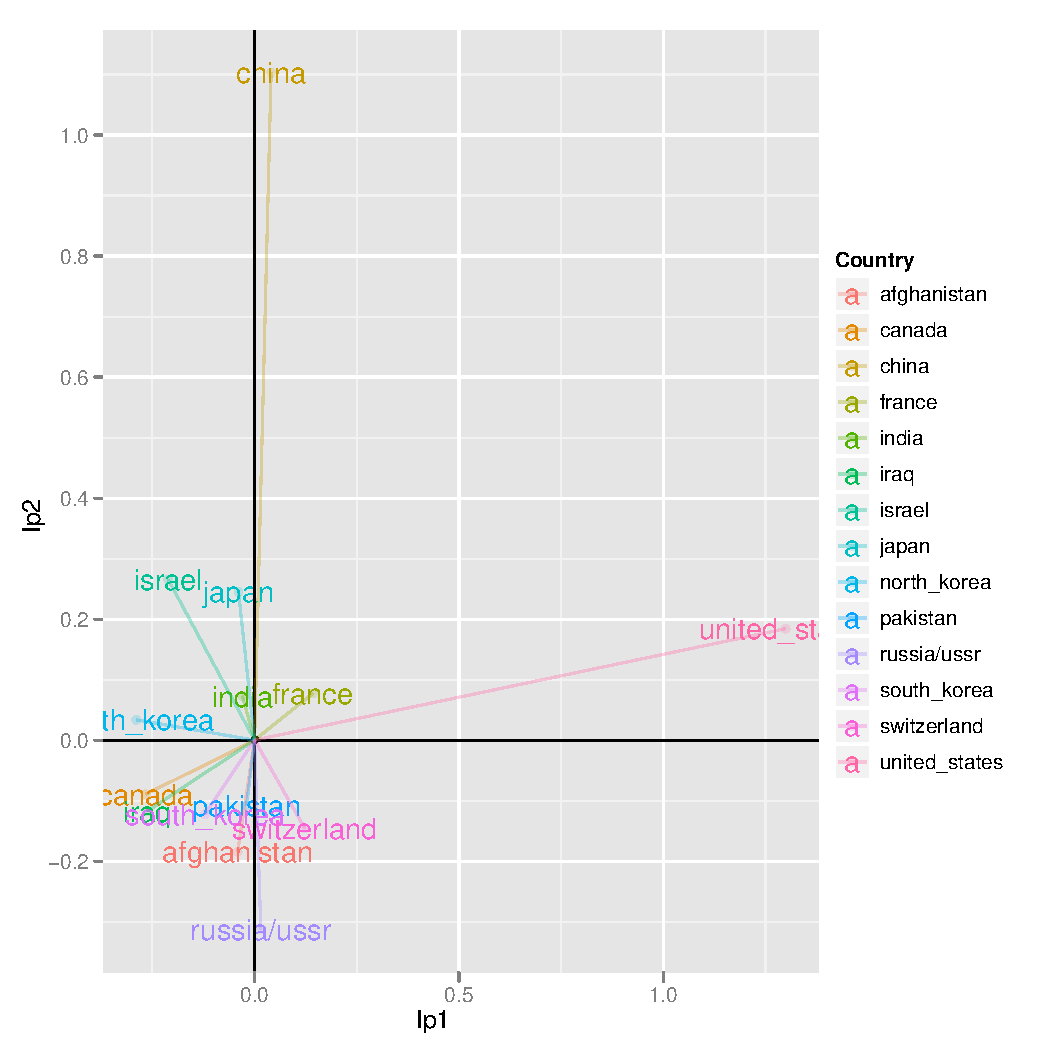
\includegraphics[width=0.33\textwidth]{chapter_foreign_relations/figures/002_countries_by_ip_2007.pdf} &
    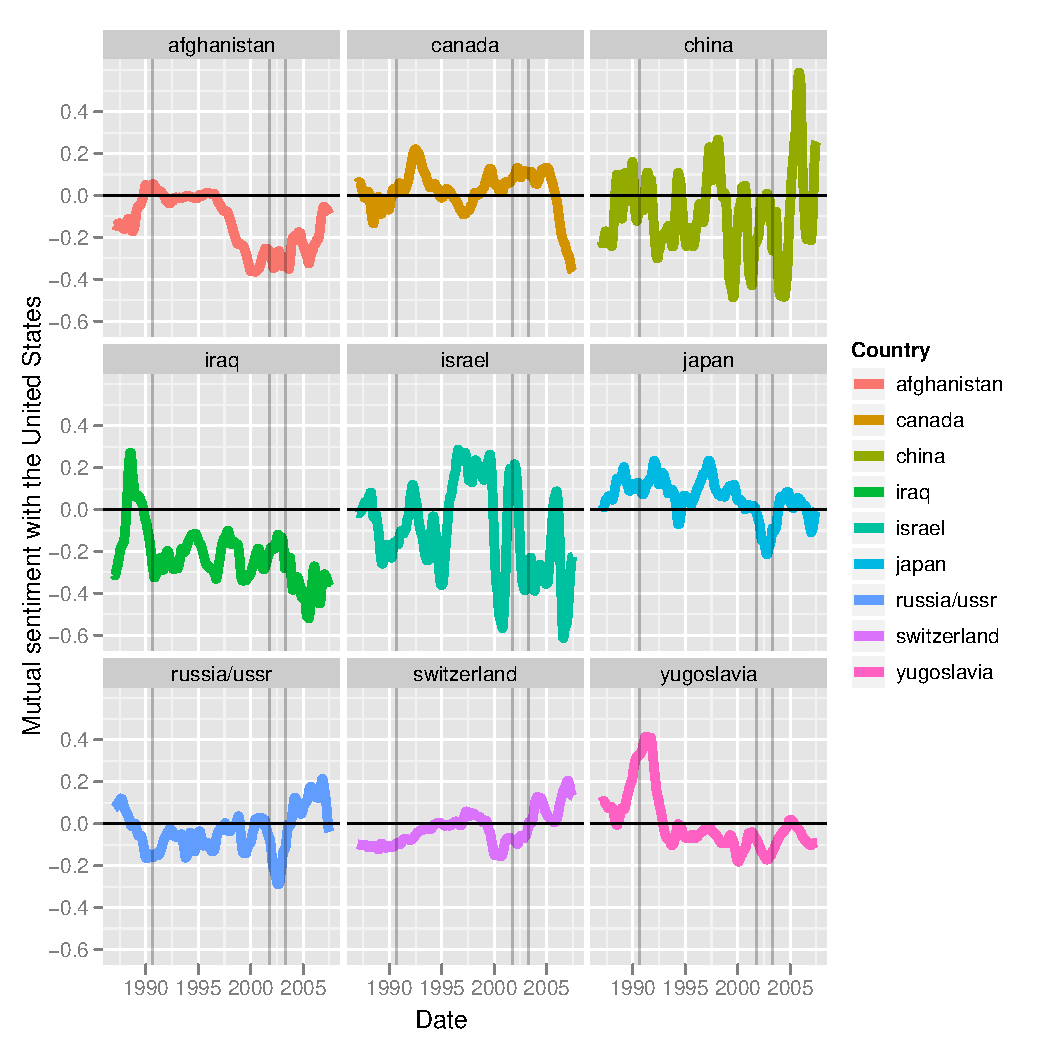
\includegraphics[width=0.33\textwidth]{chapter_foreign_relations/figures/002_us_vs_everyone.pdf} \\
    (a) & (b) & (c) \\
  \end{tabular}
  \caption{
    (a) Example positions of selected countries in the latent space of national sentiment, in 1987. Sentiment is given by the inner product between two vectors.
    (b) Example positions of selected countries in 2007.
    (c) Mutual sentiment $s = \bar x_{c, \cdot}^T \bar x_{\mbox{\small us}, \cdot}$ with the United States over time. The two Iraq wars and September 11th, 2001 are marked.
  }
  \label{figure:figures}
\end{figure}

\subsection{Results}

\paragraph{Prediction.}
For two nations $c_1$ and $c_2$ mentioned together at time $t$, we
predict their sentiment to be $\tilde s_{c_1, c_2} = \bar x_{c_1,t}
\bar x_{c_2, t}$.  Based on this estimate, the average squared error
for heldout nations is 2.32 ($R^2=0.51$), considerably better than a
baseline of text regression, which had means-squared-error $5.53$; for
comparison, average \emph{inter-rater squared error} -- the minimum
theoretically possible given the set of Mechanical Turk ratings -- was
$1.77$, and the square of the difference \emph{between} raters was
$7.11$.  We also found that using ``pseudo observations'' with even
modest observation variance improves predictive performance; these
results are summarized in Table~\ref{figure:sse_test}.

\paragraph{Static latent space.}
We first evaluate the latent-space assumption that countries'
interactions can be summarized by their positions in a latent space.
For this, we used a simplified model of sentiment, in which documents'
mean positions $\bar x_c, y_c$ are fixed, and that the sentiment is
drawn from .

We tested this assumption for both a distance and inner-product link
function, with intercepts and without intercepts.  We find that the
the inner-product assumption $\bar x_{c_1}^T \bar x_{c_2}$ alone is
poor because it provides no natural way to model mischief-prone
countries well.  If the inner-product model is endowed with intercepts
$y_{c_1}, y_{c_2}$, however, it becomes a top-performer.

Both the inner product and distance link functions perform best when
they are able to use intercepts and when they have many dimensions: we
evaluated the models with up to 9 dimensions, and they TODO(sgerrish), modeling articles' sentiment at 0.32.

\paragraph{The benefit in adding Markov drift.}
We can improve the predictive power of this model by adding a time
dimension, allowing $\bar x_c$ to drift over time for each country
$c$.  We illustrate these results in (bottom).

The inner product model again performed poorly, often worse than the
baseline model.  In this case, the seven-dimensional distance link
function performed better than any other model, and adding per-country
intercepts $y_c$ significantly \emph{hurt} the model's performance.

The better performance of these models under a time-series assumption
provides support for the argument that countries' relationships change
over time, and that these relationships are observed through the news
cycle.

\paragraph{Improvement due to zero-reversion regularization}
We can improve the predictive power of this model by adding a time
dimension, allowing $\bar x_c$ to drift over time for each country
$c$.  We illustrate these results in (bottom).

The inner product model again performed poorly, often worse than the
baseline model.  In this case, the seven-dimensional distance link
function performed better than any other model, and adding per-country
intercepts $y_c$ significantly \emph{hurt} the model's performance.

The better performance of these models under a time-series assumption
provides support for the argument that countries' relationships change
over time, and that these relationships are observed through the news
cycle.

\paragraph{Static latent space.}


\begin{figure}
%%   \begin{tabular}{|c|c|c|c|c|c|c|c|}
%%    \hline
%%   Link $\mathcal{F}(\bm x_{c_1}, y_{c_1}, \bm x_{c_2}, y_{c_2})$ & & & & & & \\
%%   \hline
%%   \textbf{Dimension of $\bm x$} & 0 & 1 & 2 & 3 & 4 & 5 & 6 & 7 & 8 & 9 \\
%%   \hline
%%   $y_{c_1} + y_{c_2}$ & 0.0964 & - & - & - & - & - & - & - & - & - \\
%%   \hline
%%   $\bm x_{c_1}^T \bm x_{c_2}$
%%   & 0.1036 & 0.1013 & 0.1050 & 0.1038 & 0.1033 & 0.1025 & 0.1018 & & & \\
%%   \hline
%%   $y_{c_1} + y_{c_2} + \bm x_{c_1}^T \bm x_{c_2}$
%%   & 0.0964 & 0.0943 & 0.0940 & 0.0936 & 0.0935 & 0.0934 & 0.0934 & & & \\
%%   \hline
%%   $-\log(||\bm x_{c_1} - \bm x_{c_2}||_2^2 + 1)$
%%   & 0.1036 & 0.1037 & 0.0978 & 0.0957 & 0.0951 & 0.0947 & 0.0943 & & & \\
%%   \hline
%%   $y_{c_1} + y_{c_2} -\log(||\bm x_{c_1} - \bm x_{c_2}||_2^2 + 1)$
%%   & 0.0964 & 0.0949 & 0.0943 & 0.0938 & 0.0939 & 0.0937 & 0.0936 & & & \\
%%   \hline
%%   mean($\{s_d\}_d$) & 0.1036 & - & - & - & - & - & - & & & \\
%%   \hline
%%   \end{tabular}
%%   \vspace{30pt}
%%   \begin{tabular}{|c|c|c|c|c|c|c|c|}
%%    \hline
%%   Link $\mathcal{F}(\bm x_{c_1}, y_{c_1}, \bm x_{c_2}, y_{c_2})$ & & & \\
%%   \hline
%%   \textbf{Dimension of $\bm x$} & 0 & 1 & 2 & 3 & 4 & 5 & 6 \\
%%   \hline
%%   $y_{c_1} + y_{c_2}$ & 0.0964 & - & - & - & - & - & - \\
%%   \hline
%%   $\bm x_{c_1}^T \bm x_{c_2}$
%%   & 0.1036 & 0.1013 & 0.1050 & 0.1038 & 0.1033 & 0.1025 & 0.1018 \\
%%   \hline
%%   $y_{c_1} + y_{c_2} + \bm x_{c_1}^T \bm x_{c_2}$
%%   & 0.0964 & 0.0943 & 0.0940 & 0.0936 & 0.0935 & 0.0934 & 0.0934 \\
%%   \hline
%%   $-\log(||\bm x_{c_1} - \bm x_{c_2}||_2^2 + 1)$
%%   & 0.1036 & 0.1037 & 0.0978 & 0.0957 & 0.0951 & 0.0947 & 0.0943 \\
%%   \hline
%%   $y_{c_1} + y_{c_2} -\log(||\bm x_{c_1} - \bm x_{c_2}||_2^2 + 1)$
%%   & 0.0964 & 0.0949 & 0.0943 & 0.0938 & 0.0939 & 0.0937 & 0.0936 \\
%%   \hline
%%   mean($\{s_d\}_d$) & 0.1036 & - & - & - & - & - & - \\
%%   \hline
\begin{tabular}{m{2cm}cc}
  \tiny{Correlates of War} & 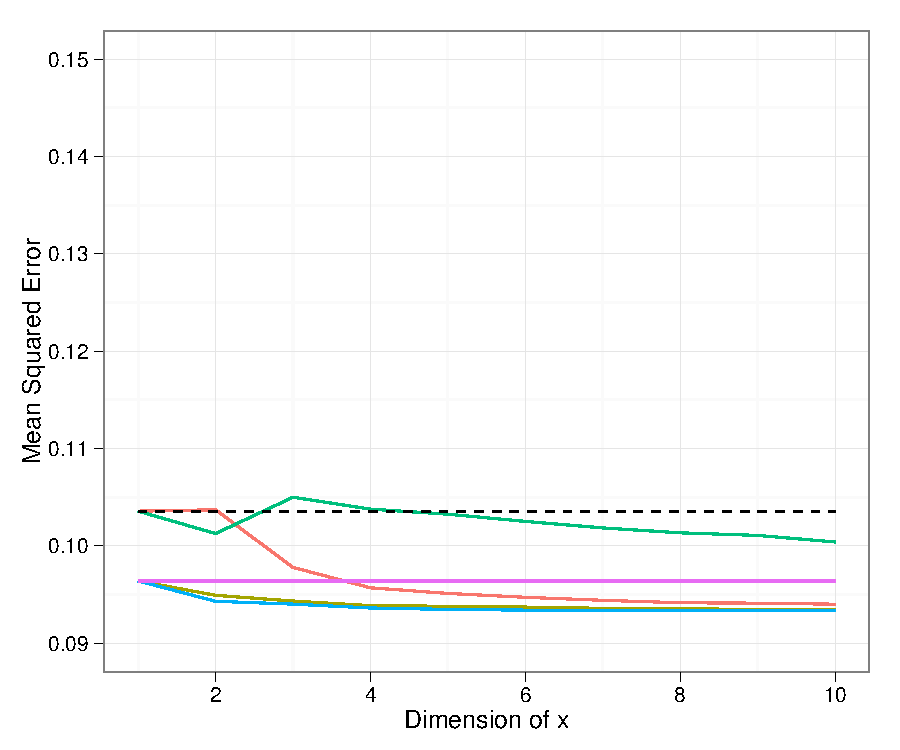
\includegraphics[height=0.2\textheight]{chapter_foreign_relations/figures/008_static_model_results.pdf} & 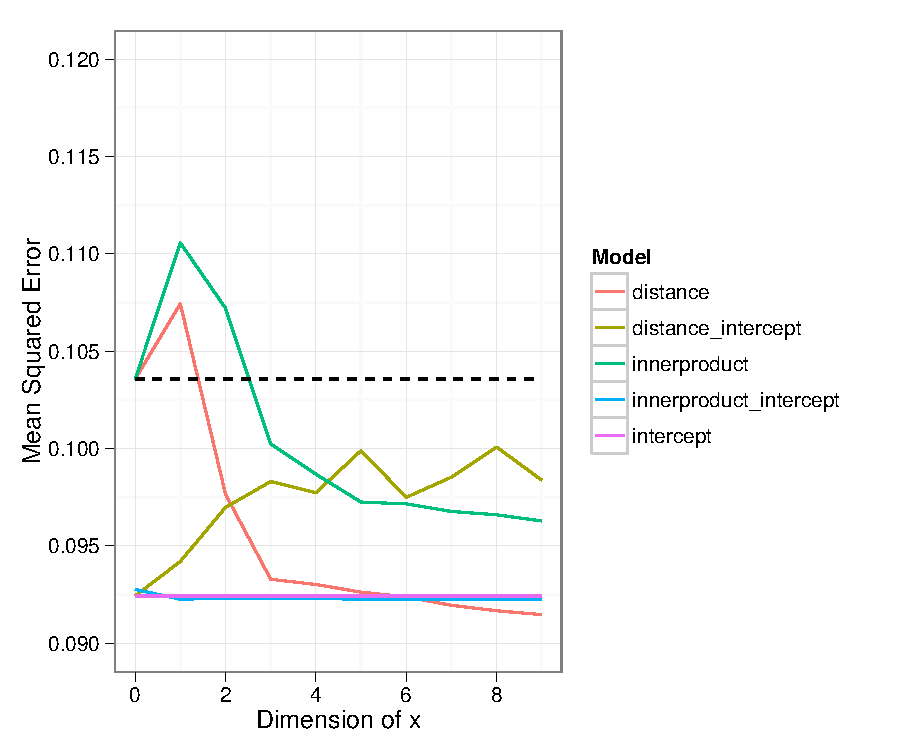
\includegraphics[height=0.2\textheight]{chapter_foreign_relations/figures/009_dynamic_model_results.pdf} \\
  \tiny{Mechanical Turk} & 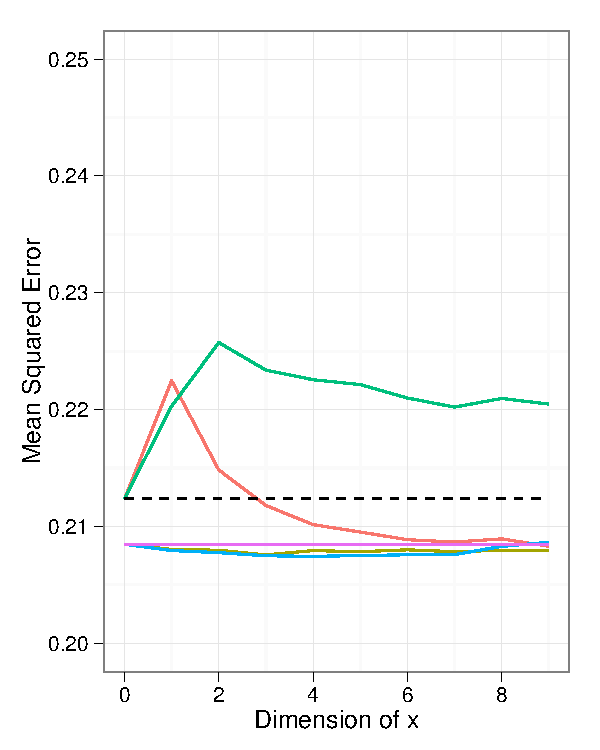
\includegraphics[height=0.2\textheight]{chapter_foreign_relations/figures/010_static_model_results.pdf} & 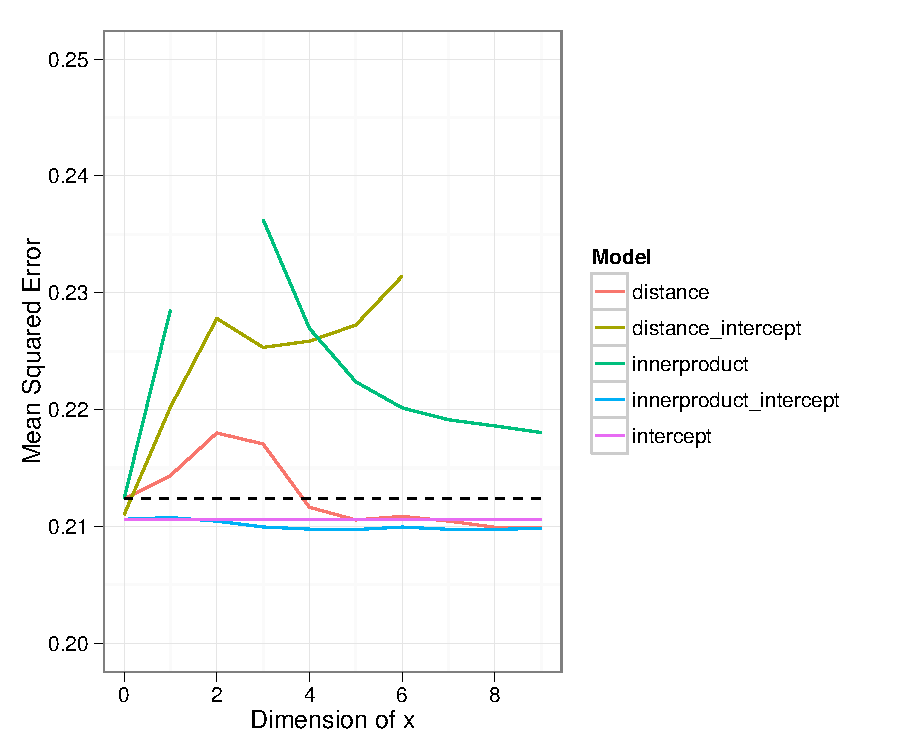
\includegraphics[height=0.2\textheight]{chapter_foreign_relations/figures/010_dynamic_model_results.pdf}
  \\ & Static & Dynamic (Interaction over time) \\
\end{tabular}
   \caption{The dyadic sentiment model captures text well . Each
     colored line represents performance of the model on a collection
     of heldout documents across twenty years of New York Times
     articles. An inner-product model with four dimensions (plus
     intercepts) performs well for most settings.  Using a dynamic
     model instead of a static model improves performance slightly }
\end{figure}

Nations' positions are illustrated in Figure~\ref{figure:figures}.
Figures~\ref{figure:figures}(a,b) show nations' relative positions
and interactions for a two- dimensional model; heldout error slightly
increased for higher dimensions. The United States' relationship with
Iraq (see Figure~\ref{figure:figures}(c)) serves as an excellent
example of this model in action; the relationship between these
nations degrades during both the Gulf War and the invasion of Iraq
following September 9th, 2001.  Israel's relationship with the United
States demonstrates one of the model's downfalls: while Israel is
considered a close ally of the United States, the raters' 95 ratings
of these nations' mentions had mean 0.12 and standard deviation
2.65.  Because the model is only as good as its ratings, the nations
appear to have a rocky relationship.

% > a = read.csv("../../data/v4/v4-doc-training_samples.csv", as.is=TRUE, header=FALSE)


  %  We then evaluate perplexity
 % \begin{align}
 %   \mbox{perp}_d & = \mathcal{E_{\hat D}} \log p(w | \bar x_{d_{c1}}
 %     \bar x_{d_{c2}} ) \\
 %     & = \frac{1}{N} \sum_N \sum_{W_{d_n}}
 %     \log p(w | \bar x_{d_{c1}} \bar x_{d_{c2}} ) \\
 % \end{align}

% \subsubsection*{Bivariate change point detection}
% In addition to identifying the latent positions of nations over
% time, we can pinpoint periods of great change or upheaval.  Sudden
% changes in a nation's position is an indication of newsworthy events
% in its history; simultaneous changes in two nations' positions is an
% indication that they are both taking part in these newsworthy events.

% The task of identifying sudden changes in a time-series is known as
% change point detection.  Change point detection is frequently
% addressed by simple univariate significance tests.  We consider
% changes in the statistic $\bar s_{c1,c2} := \bar x_{c1} \bar x_{c2}$
% (see Equation~\ref{figure:sentiment}).  Because $\bar s_{c1,c1}$ may
% be change significantly when either $x_{c_1}$ or $x_{c_2}$ changes, we
% search for simultaneous significant changes in $\bar x_{c_1}$, $\bar
% x_{c_2}$, and $\bar s_{c1,c2}$ (Note that $\mathcal{E}[s_{c1,c2}] \neq
% \bar s_{c1,c2}$; we compute $\bar s_{c1,c2}$ out of convenience.

